\documentclass[tikz,border=8pt]{standalone}
% Shared look for every TikZ diagram. Load with \input{../../tools/tikz-style.tex}
\usepackage[T1]{fontenc}
\usepackage{lmodern}
\renewcommand{\sfdefault}{lmr}  % diagrams use the same serif as the text
\usetikzlibrary{arrows.meta, positioning, shapes.geometric, calc, fit, backgrounds}
\definecolor{cblue}{HTML}{4C78A8}
\definecolor{corange}{HTML}{F58518}
\definecolor{cgreen}{HTML}{54A24B}
\definecolor{cred}{HTML}{E45756}
\definecolor{cpurple}{HTML}{B279A2}
\definecolor{cgrey}{HTML}{6B6B6B}
\tikzset{
  every picture/.style={font=\sffamily, line width=1.2pt},
  box/.style={draw=#1, fill=#1!12, rounded corners=4pt, align=center, inner sep=7pt, minimum height=1.1cm},
  box/.default=cgrey,
  arrow/.style={-{Stealth[length=3mm]}, draw=cgrey, line width=1.4pt},
  title/.style={font=\sffamily\bfseries\Large},
  note/.style={font=\sffamily\small, text=cgrey, align=center},
}
\AtBeginDocument{\hyphenpenalty=10000 \exhyphenpenalty=10000}

\begin{document}
% Section 9: Bahdanau et al.'s bidirectional encoder. A forward RNN (below) and a backward RNN (above) read the
% same words; h_j joins their two states at position j, so it summarises the words before and after word j.
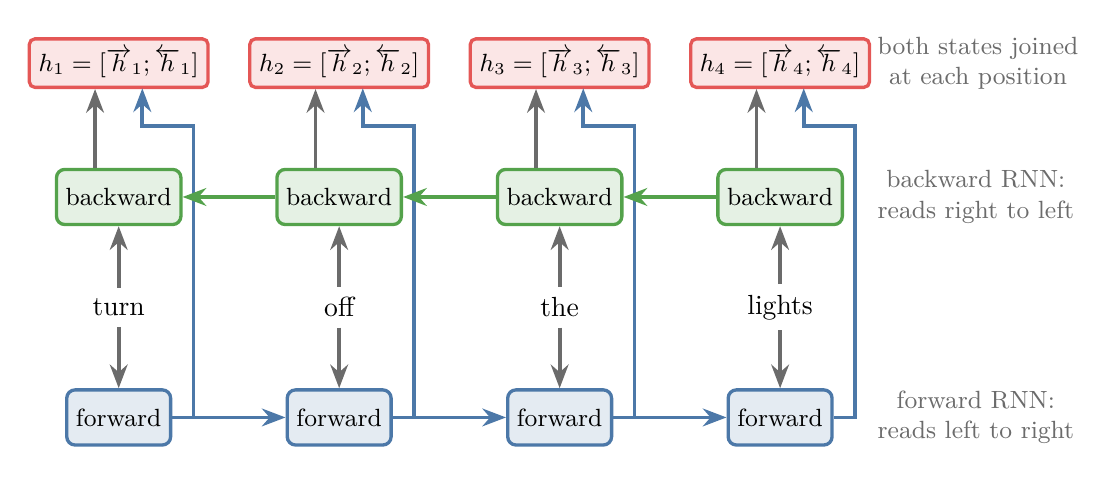
\begin{tikzpicture}[cell/.style={draw=#1, fill=#1!15, minimum width=1.2cm, minimum height=0.7cm, rounded corners=3pt, font=\sffamily\small},
  word/.style={font=\sffamily}]
  \foreach \w [count=\j] in {turn, off, the, lights} {
    \pgfmathsetmacro{\x}{2.8*\j}
    \node[word] (x\j) at (\x, 0) {\w};
    \node[cell=cblue] (f\j) at (\x, -1.4) {forward};
    \node[cell=cgreen] (b\j) at (\x, 1.4) {backward};
    \node[draw=cred, fill=cred!15, rounded corners=2pt, font=\sffamily\small] (h\j) at (\x, 3.1) {$h_\j = [\overrightarrow{h}_\j; \overleftarrow{h}_\j]$};
    \draw[arrow] (x\j) -- (f\j);
    \draw[arrow] (x\j) -- (b\j);
    \draw[arrow] ([xshift=-0.3cm]b\j.north) -- ([xshift=-0.3cm]b\j.north |- h\j.south);
    \draw[arrow, draw=cblue] (f\j.east) -- (\x + 0.95, -1.4) -- (\x + 0.95, 2.3) -- (\x + 0.3, 2.3) -- (\x + 0.3, 2.78);
  }
  \foreach \i/\j in {1/2, 2/3, 3/4} {\draw[arrow, draw=cblue] (f\i) -- (f\j); \draw[arrow, draw=cgreen] (b\j) -- (b\i);}
  \node[note, anchor=west] at (12.3, -1.4) {forward RNN:\\reads left to right};
  \node[note, anchor=west] at (12.3, 1.4) {backward RNN:\\reads right to left};
  \node[note, anchor=west] at (12.3, 3.1) {both states joined\\at each position};
\end{tikzpicture}
\end{document}
